\documentclass[
    12pt,
    openright,
    oneside,
    a4paper,
    english,
    french,
    spanish,
    brazil
    ]{abntex2}

% --- Pacotes Básicos ---
\usepackage[T1]{fontenc}
\usepackage[utf8]{inputenc}
\usepackage{helvet} % Fonte Arial/Helvetica
\renewcommand{\familydefault}{\sfdefault} % Define a fonte sem serifa como padrão
\usepackage{graphicx}
\usepackage{microtype}
\usepackage{multirow}
\usepackage{rotating}
\usepackage{amsmath,amssymb}
\usepackage{siunitx}
\usepackage{float}

% --- Margens (ABNT: Superior/Esquerda 3cm, Inferior/Direita 2cm) ---
\usepackage[top=3cm, left=3cm, right=2cm, bottom=2cm]{geometry}

% --- Espaçamento de primeira linha (ABNT) ---
\setlength{\parindent}{1.5cm}

\newcommand{\norma}[1]{\textbf{#1}}

% --- Pacote e comando para destacar, ao longo do texto, os itens do ---
% --- roteiro (ROTEIRO_DE_ELABORAÇÃO_DO_PROJETO_ELÉTRICO...) que ainda ---
% --- não foram atendidos pelo grupo. Basta remover o \FALTA{...} ---
% --- quando o item correspondente for de fato elaborado. ---
\usepackage{xcolor}
\newcommand{\FALTA}[1]{%
  \par\noindent\fcolorbox{red}{yellow!15}{%
    \parbox{\dimexpr\linewidth-2\fboxsep-2\fboxrule}{%
      \small\textbf{[PENDENTE conforme Roteiro]:} #1}}\par\vspace{2mm}}

% --- Estilo de Cabeçalho e Rodapé (Logo superior direito, Página inferior direito) ---

\makepagestyle{estilo_personalizado}
% Cabeçalho ímpar/par: vazio no centro, vazio à esquerda, espaço de logo à direita

\makeoddhead{estilo_personalizado}{}{}{
\includegraphics[width=2.2cm]{imagens/Logo_UEM.png}}


% Rodapé ímpar/par: vazio no centro, vazio à esquerda, número da página à direita
\makeoddfoot{estilo_personalizado}{}{}{\thepage}
\makeevenfoot{estilo_personalizado}{}{}{\thepage}

% --- Títulos e Subtítulos em Negrito ---
\renewcommand{\ABNTEXchapterfont}{\sffamily\bfseries}
\renewcommand{\ABNTEXchapterfontsize}{\Large}
\renewcommand{\ABNTEXsectionfont}{\sffamily\bfseries}
\renewcommand{\ABNTEXsectionfontsize}{\large}

% --- Citações (ABNT) ---
\usepackage[alf]{abntex2cite}

% --- Arquivo de Referências (Embutido para facilidade) ---
% ATENÇÃO: referências de exemplo/placeholder -- ver nota [FALTA] nos
% elementos pós-textuais. Substituir pelos dados reais e completos.


\hypersetup{
    colorlinks=true,       % Transforma as caixas em textos coloridos
    linkcolor=black,       % Cor dos links internos (tabelas, figuras)
    citecolor=black,       % Cor das citações (pode trocar para blue se preferir)
    urlcolor=black         % Cor dos links de internet
}

% --- Informações de Capa e Folha de Rosto (Contra Capa) ---
\titulo{MEMORIAL DE CÁLCULO}
\autor{ Antonio Nicolas Irmani\\
        Gabriel Henrique da Silva\\
        Gabriel Volpato\\
        João Marcos Conti Checom\\
        Julia Fernandes Gimenes\\
        Matheus Augusto Fernandes Franco\\}
\local{Maringá -- Paraná}
\data{2026}
\orientador{Glaucio Pedro de Alcantara}
\instituicao{%
  Universidade Estadual de Maringá - UEM
  \par
  Departamento de Engenharia Química 
  \par
  Engenharia Elétrica}
\tipotrabalho{Projeto Elétrico de uma Edificação}
\preambulo{Trabalho de Conclusão de Curso apresentado ao Curso de Graduação em 
Engenharia Eletrica da Universidade Estadual de Maringá, como requisito parcial para obtenção 
do título de Bacharel em Engenharia Eletrica.}

\begin{document}

% Retira espaço extra obsoleto entre as frases.
\frenchspacing

% ----------------------------------------------------------
% ELEMENTOS PRÉ-TEXTUAIS
% ----------------------------------------------------------

% ----------------------------------------------------------
% CAPA CUSTOMIZADA
% ----------------------------------------------------------
\begin{capa}
    \begin{center}
        
        % --- Cabeçalho: Logo e Instituição ---
        % O minipage divide a parte superior em duas colunas. 
        \begin{minipage}[c]{0.2\textwidth}
            \centering
            % Quando tiver a logo, apague o comando \rule abaixo e descomente o \includegraphics
            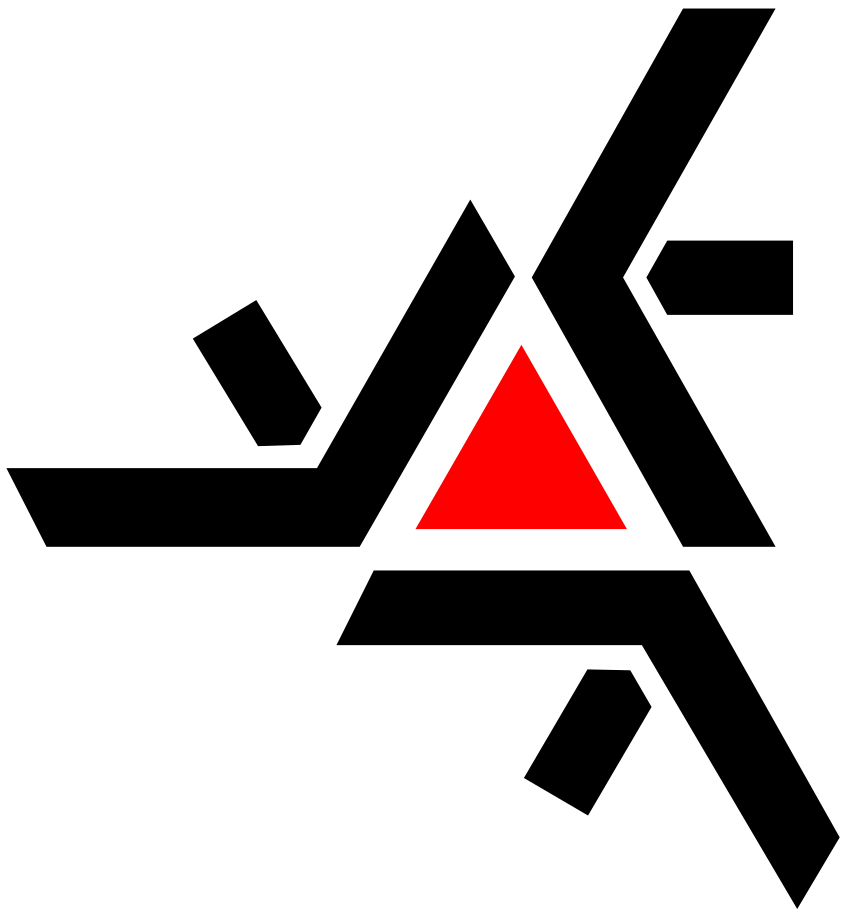
\includegraphics[width=2.8cm]{imagens/Logo.png} % Logo Capa
            %\rule{2.5cm}{3.2cm} % Retângulo preto simulando a imagem da logo
        \end{minipage}%
        \begin{minipage}[c]{0.75\textwidth}
            \centering
            \textbf{UNIVERSIDADE ESTADUAL DE MARINGÁ - UEM}\\
            \textbf{DEPARTAMENTO DE ENGENHARIA QUÍMICA}\\
            \textbf{ENGENHARIA ELÉTRICA}\\
            \textbf{INSTALAÇÕES ELÉTRICAS II - 14148}
        \end{minipage}
        
        \vspace*{3.5cm} % Espaçamento vertical até os autores
        
        % --- Lista de Autores ---
        Antonio Nicolas Irmani\\
        Gabriel Henrique da Silva\\
        Gabriel Volpato Parpineli\\
        João Marcos Conti Checom\\
        Julia Fernandes Gimenes\\
        Matheus Augusto Fernandes Franco\\
        
        \vspace*{4.5cm} % Espaçamento vertical até o título
        
        % --- Título do Trabalho ---
        \textbf{\large{INSTALAÇÃO ELÉTRICA: \\ EDIFICAÇÃO DE USO COLETIVO}}
        
        \vfill % Este comando empurra automaticamente o bloco abaixo para o limite inferior da página
        
        % --- Local e Data ---
        \textbf{MARINGÁ -- PR}\\
        \textbf{AGOSTO DE 2026}
        
    \end{center}
\end{capa}

\imprimirfolhaderosto

% ============================================================
% CONTRACAPA -- ATENÇÃO (Etapa 1 do roteiro)
% ============================================================
% O roteiro pede uma contracapa com: 1) título do trabalho; 2) uma caixa
% de texto JUSTIFICADA, ocupando da metade da página até a margem direita,
% com um texto no modelo "Parte manuscrita do Projeto elétrico residencial
% realizada pelos alunos xxxxx (...)"; 3) cidade/estado e mês/ano no
% rodapé. O comando \imprimirfolhaderosto do abntex2 gera a folha de
% rosto padrão (autor, título, natureza do trabalho, orientador), que NÃO
% corresponde ao modelo de contracapa pedido no roteiro.
\FALTA{Substituir/complementar a folha de rosto gerada por
\texttt{\textbackslash imprimirfolhaderosto} por uma \emph{contracapa}
customizada, com caixa de texto justificada da metade da página até a
margem direita, no modelo de texto sugerido pelo roteiro (ex.: "Parte
manuscrita do Projeto elétrico residencial realizada pelos alunos
[nomes], da [ano/série] série do curso de [curso], apresentado na UEM --
Maringá, como forma para obtenção da nota final da disciplina") e com
cidade/estado + mês/ano no rodapé.}

% --- Sumário ---
\pdfbookmark[0]{\contentsname}{toc}
\tableofcontents*
\cleardoublepage

% ============================================================
% ETAPA 2 DO ROTEIRO -- ordem exigida:
% Agradecimentos > Lista de Figuras > Lista de Quadros > Glossário > Índice
% (numeração em algarismos romanos do item "Agradecimentos" até
% "Glossário", inclusive -- já é o padrão do abntex2 na área pré-textual)
% ============================================================

% --- Agradecimentos ---
\begin{agradecimentos}
\FALTA{Elaborar o texto de agradecimentos do grupo (item 1 da Etapa 2).}
\end{agradecimentos}
\cleardoublepage

% --- Lista de Ilustrações (Figuras) ---
\pdfbookmark[0]{\listfigurename}{lof}
\listoffigures*
\cleardoublepage
\FALTA{A Lista de Figuras está vazia porque nenhuma figura (planta baixa,
fluxograma, diagrama unifilar, foto, etc.) foi inserida no corpo do
trabalho com \texttt{\textbackslash caption} em ambiente \texttt{figure}.
Inserir as figuras exigidas nas etapas seguintes (fluxograma, prumada,
diagramas unifilares) para que esta lista seja preenchida
automaticamente.}

% --- Lista de Quadros ---
% Observação de norma: em ABNT, "Tabela" = dado estatístico/numérico e
% "Quadro" = informação textual organizada em linhas/colunas (não
% numérica). O documento atual só contém Tabelas (já listadas em "Lista
% de Tabelas", abaixo); se o grupo decidir usar Quadros (ex.: quadro-
% resumo de normas, quadro de etapas do projeto), a Lista de Quadros
% deve ser criada com o ambiente \texttt{quadro} do abntex2
% (\texttt{\textbackslash listofquadros}).
\phantomsection
\addcontentsline{toc}{chapter}{Lista de Quadros}
\pdfbookmark[0]{Lista de Quadros}{loq}
\chapter*{Lista de Quadros}
\FALTA{Nenhum Quadro (ambiente \texttt{quadro} do abntex2, distinto de
\texttt{table}) foi criado até o momento -- apenas Tabelas. Definir se o
grupo utilizará Quadros (ex.: quadro-resumo dos Princípios Fundamentais
da NBR 5410 \cite{nbr5410}, quadro do esquema de distribuição) e, em caso positivo,
gerar esta lista com \texttt{\textbackslash listofquadros}.}
\cleardoublepage

% --- Glossário ---
%\begin{glossario}
\begin{itemize}[leftmargin=1.2cm]
    \item[NBR] Norma Brasileira, publicada pela ABNT.
    \item[COPEL] Companhia Paranaense de Energia, concessionária de energia
    elétrica do Estado do Paraná.
    \item[TUG] Tomada de Uso Geral.
    \item[TUE] Tomada de Uso Específico.
    \item[QGBT] Quadro Geral de Baixa Tensão.
\end{itemize}
\FALTA{Completar o glossário com os demais termos técnicos utilizados no
memorial (ex.: DTM, IDR/DR, NTC, demanda, fator de potência, prumada,
esquema de distribuição TN/TT/IT, etc.).}
%\end{glossario}
\cleardoublepage

% --- Lista de Tabelas ---
\pdfbookmark[0]{\listtablename}{lot}
\listoftables*
\cleardoublepage

% --- Índice ---
\phantomsection
\addcontentsline{toc}{chapter}{Índice}
\pdfbookmark[0]{Índice}{idx}
\chapter*{Índice}
\FALTA{O Índice remissivo ainda não foi gerado. É necessário: 1) carregar
o pacote \texttt{makeidx} (\texttt{\textbackslash usepackage\{makeidx\}}
e \texttt{\textbackslash makeindex}) no preâmbulo; 2) marcar os termos
relevantes ao longo do texto com \texttt{\textbackslash index\{termo\}}
(ex.: \texttt{\textbackslash index\{fator de demanda\}}); 3) inserir
\texttt{\textbackslash printindex} nos elementos pós-textuais; e 4)
compilar o projeto com o utilitário \texttt{makeindex} além do
\texttt{pdflatex}.}
\cleardoublepage

% ----------------------------------------------------------
% ELEMENTOS TEXTUAIS
% ----------------------------------------------------------
\textual
% Ativa o cabeçalho/rodapé personalizado para o texto
\pagestyle{estilo_personalizado}
\aliaspagestyle{chapter}{estilo_personalizado}

% NOTA SOBRE ALINHAMENTO: 
% O padrão ABNT exige texto justificado. A capa e títulos já são centralizados por padrão na classe abntex2.
% Se você desejar que o corpo dos parágrafos do texto também fique centralizado (fora da norma padrão), 
% basta descomentar o comando \centering abaixo:
% \centering




% ============================================================
% ETAPA 3 DO ROTEIRO -- INTRODUÇÃO
% ============================================================
\section{Introdução}

\subsection{Motivação}

\hspace{1.27cm}A elaboração de um projeto elétrico completo para uma edificação de uso
coletivo permite consolidar, em um único estudo de caso, os principais
critérios normativos de dimensionamento de instalações elétricas de baixa
tensão previstos na ABNT NBR 5410, além de aproximar a formação do
engenheiro eletricista das rotinas efetivamente praticadas junto às
concessionárias de energia elétrica (no caso, a COPEL) para a obtenção do
fornecimento de energia de uma edificação multifamiliar.
\FALTA{Personalizar este parágrafo com a motivação específica do grupo
para a escolha da edificação/estudo de caso (por exemplo: relevância do
tema para a formação profissional, características que tornam o projeto
desafiador -- número de pavimentos, presença de cargas especiais,
necessidade de subestação, etc.).}

\subsection{Definições de Projetos Elétricos}

\hspace{1.27cm}Um projeto elétrico é o conjunto de documentos técnicos -- memorial
descritivo e de cálculo, plantas, diagramas unifilares e especificações --
que define, de forma completa e auditável, todos os componentes de uma
instalação elétrica (condutores, eletrodutos, dispositivos de manobra e
proteção, quadros de distribuição e, quando aplicável, subestação e grupo
gerador), assegurando que a instalação atenda simultaneamente aos
requisitos de segurança de pessoas e bens, de funcionamento adequado ao uso
a que se destina e de conservação dos bens, nos termos estabelecidos pela
ABNT NBR 5410.

\subsection{Definições das Unidades Consumidoras}

\hspace{1.27cm}Unidade consumidora é o conjunto de instalações e equipamentos elétricos
caracterizado pelo recebimento de energia elétrica em um só ponto de
entrega, com medição individualizada e correspondente a uma única
classe/subclasse de consumo, nos termos definidos pela concessionária de
energia elétrica local.
\FALTA{Detalhar aqui as definições de unidade consumidora, categoria de
fornecimento (residencial, comercial, condomínio) e classificação adotadas
especificamente pela concessionária de energia elétrica em questão
(COPEL), com base na Norma Técnica COPEL (NTC) aplicável, conforme exigido
no item 1.3 da Etapa 3 do roteiro.}

% ============================================================
% ETAPA 4 DO ROTEIRO -- DESCRIÇÃO DAS ETAPAS DO PROJETO
% ============================================================
\section{Descrição das Etapas do Projeto}

A execução deste projeto foi baseada nas plantas baixas de arquitetura
distribuídas pelo professor (formato DWG), a partir das quais foram
extraídos os perímetros e áreas de cada ambiente (Tabela~\ref{tab:apartamento_individual}).

\FALTA{Inserir aqui um fluxograma sequencial (figura) com as etapas de
elaboração do projeto -- por exemplo: Levantamento de plantas
$\rightarrow$ Levantamento de Cargas $\rightarrow$ Cálculo de Potências e
Carga Total $\rightarrow$ Cálculo de Demanda $\rightarrow$ Definição da
Categoria/Tipo de Fornecimento $\rightarrow$ Dimensionamento de Circuitos,
Condutores e Eletrodutos $\rightarrow$ Dimensionamento da Proteção
$\rightarrow$ Prumada Elétrica e Diagramas Unifilares $\rightarrow$ Pedido
de Fornecimento à COPEL -- conforme pedido no item 1 da Etapa 4 do
roteiro ("de preferência com fluxograma sequencial").}

\subsection{Apresentação e Finalidade do Projeto}

\hspace{1.27cm}Este memorial tem por objetivo apresentar, de forma técnica e sequencial, a
metodologia de cálculo empregada no dimensionamento do sistema elétrico de
uma edificação de uso coletivo, contemplando desde o levantamento de cargas
até a especificação final dos dispositivos de proteção, condutores e,
quando aplicável, da subestação e do grupo gerador.

Com base nas plantas baixas fornecidas e no levantamento apresentado na
Tabela~\ref{tab:apartamento_individual}, tem-se as seguintes características gerais da
edificação em estudo:

\begin{itemize}[leftmargin=1.2cm]
    \item A edificação em estudo é residencial multifamiliar, composta por
    apartamentos-tipo com área privativa de \textbf{89,3~m²} cada
    (Tabela~\ref{tab:apartamento_individual}), organizados em \textbf{14 unidades
    autônomas} distribuídas em pavimentos, agrupadas em \textbf{2 Centros
    de Medição} (CM1, com 5 apartamentos, e CM2, com 9 apartamentos),
    conforme detalhado na Tabela~7 (Cargas dos Apartamentos);
    \FALTA{confirmar/ajustar a natureza exata da edificação -- ex.:
    edifício residencial puro ou de uso misto -- e sua classificação de
    ocupação conforme a concessionária local e a NBR~5410;}
    \item A área construída total do apartamento-tipo é de
    \textbf{89,3~m²} (Tabela~\ref{tab:apartamento_individual}); a área construída total da
    edificação (soma das 14 unidades autônomas mais áreas comuns) ainda
    precisa ser consolidada;
    \FALTA{informar a área construída total da edificação (m²), incluindo
    áreas comuns, e o número de pavimentos e blocos;}
    \item A finalidade do documento é demonstrar, de maneira auditável, que
    o dimensionamento atende simultaneamente aos critérios de
    \emph{capacidade de condução de corrente}, \emph{queda de tensão} e
    \emph{proteção contra sobrecorrentes e contatos indiretos}, tal como
    exigido pela ABNT NBR 5410;
    \item Os ambientes contemplados no levantamento de cargas de cada
    apartamento-tipo são os treze cômodos listados na
    Tabela~\ref{tab:apartamento_individual} (Área de Serviço, BWC, Cozinha, Sala, Quarto
    1, Circulação, Suíte, WC Suíte, Quarto 2, WC Social e Sacadas 1 a 3),
    pois é a partir da classificação de cada ambiente que a norma define os
    critérios mínimos de iluminação, tomadas e proteção diferencial a
    serem aplicados;
    \FALTA{incluir também os ambientes de uso comum (hall, casa de
    máquinas, subestação, guarita, etc.) no levantamento, necessários para
    a Carga do Condomínio (subseção~\ref{subsec:carga_condominio}).}
\end{itemize}



% ============================================================
\subsection{Normas de Referência}

\hspace{1.27cm}O dimensionamento apresentado neste memorial fundamenta-se, prioritariamente,
na \norma{ABNT NBR 5410:2004} -- \emph{Instalações elétricas de baixa
tensão} -- documento normativo que estabelece as condições mínimas a serem
atendidas por instalações elétricas de baixa tensão, de modo a garantir:

\begin{enumerate}[leftmargin=1.2cm]
    \item o funcionamento adequado da instalação e a segurança de pessoas e
    animais domésticos (proteção contra choques elétricos, efeitos térmicos
    e sobrecorrentes);
    \item o funcionamento correto da instalação para o uso a que se destina;
    \item a conservação de bens.
\end{enumerate}

A NBR 5410 é a base normativa para os seguintes blocos deste memorial, cuja
correspondência é explicitada ao longo do texto:

\begin{itemize}[leftmargin=1.2cm]
    \item \textbf{Seção 3 (Levantamento de Cargas)} -- critérios mínimos de
    potência para iluminação e tomadas de uso geral, tratados na norma no
    âmbito da determinação da \emph{carga instalada} e dos \emph{critérios
    de previsão de pontos de utilização} em instalações residenciais e
    similares;
    \item \textbf{Seção 4 e 5 (Potências e Demanda)} -- conceitos de
    \emph{fator de potência}, \emph{fator de demanda} e \emph{fator de
    utilização}, empregados para evitar o superdimensionamento de
    condutores e dispositivos de proteção;
    \item \textbf{Seção 7 (Dimensionamento de Circuitos)} -- critérios de
    determinação da corrente de projeto e dos fatores de correção por
    agrupamento de circuitos e por temperatura ambiente, tabelados na norma;
    \item \textbf{Seção 8 (Condutores e Eletrodutos)} -- seções mínimas de
    condutores por finalidade de circuito e taxa máxima de ocupação de
    eletrodutos;
    \item \textbf{Seção 9 (Dispositivos de Proteção)} -- coordenação entre
    disjuntores termomagnéticos, dispositivos DR e a capacidade de condução
    de corrente dos condutores, segundo a condição geral de proteção contra
    sobrecargas.
\end{itemize}

Adicionalmente, sempre que a edificação coletiva possuir \textbf{subestação
transformadora própria} (cabine primária), com fornecimento em média tensão
pela concessionária, aplica-se de forma complementar a \norma{ABNT NBR
14039 \cite{nbr14039}:2005} -- \emph{Instalações elétricas de média tensão de 1,0 kV a
36,2 kV}, que disciplina o dimensionamento dos equipamentos de manobra e
proteção em média tensão, a malha de aterramento da subestação e os ajustes
dos relés de proteção do transformador.

Complementarmente, e sem prejuízo da precedência da NBR 5410, este memorial
observa também os padrões técnicos e critérios de fornecimento da
concessionária local de energia elétrica, os quais definem, entre outros
aspectos, o tipo de ligação (mono, bi ou trifásica), os limites de demanda
por tipo de fornecimento e as exigências construtivas para entrada de
serviço e subestação.

% ============================================================
\subsection{Levantamento de Cargas (Dimensionamento e Quantitativo)}

\hspace{1.27cm}Nesta seção demonstra-se, ambiente a ambiente, como foi obtida a potência
instalada de cada ponto de utilização, em estrita observância aos critérios
mínimos normativos -- que constituem \emph{piso obrigatório}, podendo o
projetista adotar valores superiores sempre que a carga real dos
equipamentos previstos assim o exigir.

\begin{table}[H]
\centering
\caption{Informações de Apartamento Individual}

% --- AJUSTES DE ESPAÇAMENTO ---
\renewcommand{\arraystretch}{1.4} % Aumenta a altura das linhas (padrão é 1.0)
\setlength{\tabcolsep}{12pt}      % Aumenta o espaço lateral entre as colunas (padrão é 6pt)
% ------------------------------

\begin{tabular}{c c c}
\toprule
\textbf{Cômodos} & \textbf{Perímetro} \small{(m)} & \textbf{Área} \small{(m²)} \\
\toprule
Área de Serviço	& 6,9     & 2,8 \\
BWC	            & 6,3     & 2,15 \\
Cozinha	        & 9,85    & 5,97 \\
Sala	        & 17,56   & 17,72 \\
Quarto 1	    & 11,9    & 8,78 \\
Circulação	    & 7,7     & 3,38 \\
Suíte           & 14,2    & 12,51 \\
WC Suíte        & 8,4     & 3,85 \\
Quarto 2        & 12,8    & 9,88 \\
WC Social       & 7,9     & 3,51 \\
Sacada 1        & 13,2    & 10,34 \\
Sacada 2        & 8,9     & 4,63 \\
Sacada 3        & 7,6     & 3,75 \\\toprule
\textbf{Total}  & \textbf{133,2}   & \textbf{89,3} \\\toprule
\end{tabular}
\fonte{O autor (2026).}
\label{tab:apartamento_individual}
\end{table}

\subsubsection{Iluminação}

\hspace{1.27cm} A NBR 5410 estabelece critérios mínimos de potência para pontos de
iluminação em função da área do ambiente, de modo a assegurar um nível de
carga compatível com o uso residencial e similar, ainda que a definição
luminotécnica final (número de luminárias, fluxo luminoso, iluminância em
lux) deva ser objeto de projeto luminotécnico específico, com base na
ABNT NBR ISO/CIE 8995.

\textbf{Critério mínimo de potência (carga instalada de iluminação):}

\begin{equation}
    P_{ilum} =
    \begin{cases}
        \SI{100}{VA}, & \text{se } A \le \SI{6}{\meter\squared} \\[4pt]
        \SI{100}{VA} + \SI{60}{VA}\cdot n, & \text{se } A > \SI{6}{\meter\squared}
    \end{cases}
    \label{eq:iluminacao}
\end{equation}

em que $A$ é a área do ambiente e $n$ é o número de acréscimos de
\SI{4}{\meter\squared} \emph{inteiros} que excedem os \SI{6}{\meter\squared}
iniciais (frações de \SI{4}{\meter\squared} não geram acréscimo adicional).

Complementarmente, para fins de posicionamento do ponto de luz e verificação
de distâncias mínimas a obstáculos (armários, prateleiras), pode-se estimar
a distância útil do foco luminoso em relação ao plano de trabalho por meio
de:

\begin{equation}
    d = b - a
    \label{eq:distancia_foco}
\end{equation}

sendo $b$ o pé-direito do ambiente e $a$ a distância entre a lâmpada/luminária
e o teto (altura de suspensão ou embutimento).

\begin{table}[H]
\centering
\caption{Iluminação - Apartamentos Individual}

% --- AJUSTES DE ESPAÇAMENTO ---
\renewcommand{\arraystretch}{1.4} % Aumenta a altura das linhas (padrão é 1.0)
\setlength{\tabcolsep}{12pt}      % Aumenta o espaço lateral entre as colunas (padrão é 6pt)
% ------------------------------

\begin{tabular}{c c c c c}
\toprule
\textbf{Cômodos} &\textbf{Quantidade} & \textbf{Potência Unitária} & \textbf{Potência Total}\\
\toprule
Área de Serviço	& 1   & 100 & 100 \\
BWC	             & 1 & 100 &  100 \\
Cozinha	         & 1 & 100 &  100 \\
Sala	          & 3 & 100 + 60 +60 &  220 \\
Quarto 1	     & 1 & 100 &  100 \\
Circulação	     & 1 & 100 &  100 \\
Suíte             & 3 & 100 + 60 + 60 &  220 \\
WC Suíte         & 1 & 100 &  100 \\
Quarto 2         & 2 & 100 + 60 &  160 \\
WC Social        & 1 & 100 &  100 \\
Sacada 1          & 2 & 100 + 60 &  160 \\
Sacada 2         & 1 & 100 &  100 \\
Sacada 3         & 1 & 100 &  100 \\\toprule
\textbf{Total}   & \textbf{19} & \textbf{1.660} &  \textbf{1.660} \\\toprule
\end{tabular}
\fonte{O autor (2026).}
\label{tab:iluminacao_apartamento_individual}
\end{table}

\FALTA{A linha "Total" desta tabela estava incorretamente repetindo os
valores de uma única linha (1, 100, 100); foi corrigida acima para o
somatório das potências individuais (\textbf{1.660~VA}). Além disso,
recomenda-se conferir os valores de \textbf{Suíte} (12,51~m², excedente de
6,51~m² sobre os 6~m² iniciais $\Rightarrow n=1 \Rightarrow$ 100+60 =
\textbf{160~VA}, e não 220~VA) e de \textbf{Quarto~2} (9,88~m², excedente
de 3,88~m² $\Rightarrow n=0 \Rightarrow$ \textbf{100~VA}, e não 160~VA)
frente à Equação~\eqref{eq:iluminacao}, pois os valores atualmente
lançados na tabela não correspondem exatamente ao critério de
arredondamento ali definido (acréscimos de \SI{4}{\meter\squared}
\emph{inteiros}). Essa verificação também impacta o total de
\textbf{1.560~W} de iluminação por apartamento indicado na Tabela "Cargas
dos Apartamentos" (Seção~4.5).}

\subsubsection{Tomadas de Uso Geral (TUGs)}

\hspace{1.27cm} O critério mínimo de quantidade de TUGs é definido pela norma em função do
\emph{perímetro} do ambiente, distinguindo-se conforme a finalidade do
cômodo, em razão da maior densidade de aparelhos eletrodomésticos esperada
em cozinhas, áreas de serviço e ambientes análogos:

\begin{itemize}[leftmargin=1.2cm]
    \item \textbf{Salas e dormitórios:} 1 tomada para cada \SI{5}{\meter} ou
    fração de perímetro, com no mínimo 1 ponto por ambiente;
    \item \textbf{Cozinhas, áreas de serviço, copas e locais análogos:} 1
    tomada para cada \SI{3,5}{\meter} ou fração de perímetro, também com no
    mínimo 1 ponto por ambiente.
\end{itemize}

\begin{equation}
    N_{TUG} = \left\lceil \dfrac{\text{Per\'imetro}}{L_{ref}} \right\rceil,
    \qquad
    L_{ref} =
    \begin{cases}
        \SI{5}{\meter}, & \text{salas e dormitórios} \\
        \SI{3,5}{\meter}, & \text{cozinhas e áreas molhadas}
    \end{cases}
    \label{eq:tug}
\end{equation}

Em áreas comuns de edificações coletivas (halls, circulações, guaritas), a
mesma lógica de perímetro deve ser aplicada, respeitando-se ainda eventuais
exigências adicionais de tomadas para limpeza e manutenção previstas em
projeto.

\begin{table}[H]
\centering
\caption{Tomadas Gerais - Apartamentos Individual}

% --- AJUSTES DE ESPAÇAMENTO ---
\renewcommand{\arraystretch}{1.4} % Aumenta a altura das linhas (padrão é 1.0)
\setlength{\tabcolsep}{12pt}      % Aumenta o espaço lateral entre as colunas (padrão é 6pt)
% ------------------------------

\begin{tabular}{c c c c c}
\toprule
\textbf{Cômodos} &\textbf{Quantidade} & \textbf{Potência Unitária} & \textbf{Potência Total}\\
\toprule
Área de Serviço	 & 1 & 600 & 600\\
BWC	             & 1 & 600 &  600\\
Cozinha	         & 3 & 600 + 600 + 600 &  1800\\
Sala	         & 4 & 100 + 100 + 100 + 100 &  400\\
Quarto 1	     & 3 & 100 + 100 + 100 &  300\\
Circulação	     & 1 & 100 &  100\\
Suíte            & 4 & 100 + 100 + 100 + 100 &  400\\
WC Suíte         & 1 & 600 &  600\\
Quarto 2         & 4 & 100 + 100 + 100 + 100 &  400\\
WC Social        & 1 & 600 &  600\\
Sacada 1         & 3 & 600 + 600 + 600 &  1800\\
Sacada 2         & 0 & 0 &  0\\
Sacada 3         & 0 & 0 &  0\\
\toprule
\textbf{Total}   & \textbf{26} & \textbf{7600} &  \textbf{7600} \\
\toprule
\end{tabular}
\fonte{O autor (2026).}
\label{tab:tomadas_gerais_apartamento_individual}
\end{table}

\subsubsection{Tomadas de Uso Específico (TUEs)}

\hspace{1.27cm} As TUEs correspondem aos pontos destinados a equipamentos fixos ou de
potência elevada e localização definida em projeto -- como aparelhos de
ar-condicionado, chuveiros e torneiras elétricas, máquinas de lavar e
secar, fornos elétricos e bombas de menor porte. Para essas cargas, a
potência do ponto \emph{não} é estimada por critério geométrico, mas sim
adotada diretamente a partir da potência nominal do equipamento informada
pelo fabricante:

\begin{equation}
    P_{TUE} = P_{nominal\ do\ equipamento} \quad [\si{W}]
    \label{eq:tue}
\end{equation}


\begin{table}[H] % <--- Força a tabela a ficar EXATAMENTE AQUI
\centering

% Inicia a rotação do conteúdo
\begin{sideways}
    % O minipage serve para "empacotar" o título e a tabela juntos para que o caption funcione virado.
    % O tamanho \textheight indica que a tabela pode ocupar até a altura máxima da página
    \begin{minipage}{\textheight}
        \centering
        \caption{Tomadas de Uso Especifico}
        \vspace{0.1cm} % Dá um espacinho entre o título e a tabela
        
        \renewcommand{\arraystretch}{1.06} % Ajusta a altura das linhas da tabela
        \setlength{\tabcolsep}{8pt}       

        \begin{tabular}{c  c c c c c}
        \toprule
        \multirow{2}{*}{\textbf{Ambiente}} & \multicolumn{5}{c}{\textbf{TUE's}} \\
        \cline{2-6} 
        & \textbf{Quant.} & \textbf{Tipo (de aparelho)} & \textbf{Potência Unitária (W)} & \textbf{Potência Total (W)} & \textbf{Potência Total (VA)} \\
        \toprule
        \multirow{2}{*}{Área de Serviço} 
        & 1 & Máquina Lava e Seca & 1220 & \multirow{2}{*}{1360} & \multirow{2}{*}{1700} \\
        & 1 & Robô Aspirador     & 140  &                       &                       \\
        \toprule
        BWC & 1 & Chuveiro & 7500 & 7500 & 9375 \\
        \toprule
        \multirow{5}{*}{Cozinha} 
        & 1 & Torneira Elétrica & 5550 & \multirow{5}{*}{12990} & \multirow{5}{*}{16237,5} \\
        & 1 & Fogão             & 4000 &                        &                          \\
        & 1 & Microondas        & 1100 &                        &                          \\
        & 1 & Geladeira         & 340  &                        &                          \\
        & 1 & Air Fryer         & 2000 &                        &                          \\
        \toprule
        Sala & 1 & A/C Central & 1500 & 1500 & 1875 \\
        \toprule 
        \multirow{2}{*}{Quarto 1} 
        & 1 & Televisão & 300 & \multirow{2}{*}{1115} & \multirow{2}{*}{1393,75} \\
        & 1 & Ar Condicionado & 815  &                       &                       \\
        \toprule
        Circulação & - & - & - & - & - \\
        \toprule
        \multirow{2}{*}{Quarto 1} 
        & 1 & Televisão & 300 & \multirow{2}{*}{1500} & \multirow{2}{*}{1800} \\
        & 1 & Ar Condicionado & 1200  &                       &                       \\
        \toprule
        WC Suíte & 1 & Chuveiro & 7500 & 7500 & 9375 \\
        \toprule
        \multirow{2}{*}{Quarto 2} 
        & 1 & Televisão & 300 & \multirow{2}{*}{1115} & \multirow{2}{*}{1393,75} \\
        & 1 & Ar Condicionado & 815  &                       &                       \\
        \toprule
        WC Social & 1 & Chuveiro & 7500 & 7500 & 9375 \\
        \toprule
        Sacada 1 & 1 & Adega & 180 & 180 & 225 \\
        \toprule
        Sacada 2 & - & - & - & - & - \\
        \toprule
        Sacada 3 & - & - & - & - & - \\
        \toprule
        \textbf{Total} & \textbf{18} & - & \textbf{42260} & \textbf{42260} & \textbf{52750} \\
        \toprule
        \end{tabular}
        
        \vspace{0.2cm}
        \fonte{O autor (2026).}
    \end{minipage}
\end{sideways}

\end{table}

\newpage

\subsubsection{Cargas Especiais de Edificações Coletivas}

\hspace{1.27cm} Nas edificações de uso coletivo, soma-se ao levantamento residencial
convencional o levantamento das \textbf{cargas de uso comum}, cuja
importância é proporcional ao porte da edificação e que, com frequência,
concentram os maiores blocos de potência instalada:

\begin{itemize}[leftmargin=1.2cm]
    \item motobombas de recalque (abastecimento de água);
    \item bombas de incêndio (sistema de combate a incêndio), cujo
    dimensionamento elétrico deve ainda observar a ABNT NBR 13714;
    \item elevadores e demais equipamentos de transporte vertical;
    \item iluminação e tomadas de áreas comuns, casa de máquinas e
    subestação;
    \item cargas de portões automáticos, cercas elétricas e sistemas de
    segurança, quando existentes.
\end{itemize}

Cada carga especial deve ser identificada individualmente, com sua potência
nominal, regime de funcionamento (contínuo, intermitente) e corrente de
partida, dado relevante para o dimensionamento dos condutores e da proteção
correspondente.

% ============================================================
\subsection{Carga dos Apartamentos}
\label{subsec:carga_apartamentos}
\hspace{1.27cm}
As potências levantadas na subseção anterior encontram-se, em sua maioria,
expressas em termos de potência aparente (VA), unidade adotada pela norma
para o levantamento de carga de iluminação e TUGs. Para a determinação da
carga instalada de cada apartamento em termos de potência ativa,
aplica-se o fator de potência (FP) característico de cada tipo de carga:

\begin{equation}
    P\,[\si{W}] = S\,[\si{VA}] \times FP
    \label{eq:potencia_ativa}
\end{equation}

Adotam-se os seguintes fatores de potência de referência, coerentes com a
prática normativa para o levantamento simplificado de cargas residenciais
e coletivas:

\begin{itemize}[leftmargin=1.2cm]
    \item Iluminação: $FP = 1{,}0$;
    \item TUGs: $FP = 0{,}80$;
    \item TUEs e cargas especiais: FP conforme dado de placa do fabricante
    do equipamento (na ausência de informação, admite-se $FP = 0{,}92$ como
    valor de referência conservador para motores e equipamentos
    monofásicos/trifásicos usuais, devendo ser substituído pelo valor real
    sempre que disponível).
\end{itemize}

\begin{table}[H] % <--- Força a tabela a ficar EXATAMENTE AQUI
\centering

% Inicia a rotação do conteúdo
\begin{sideways}
    % O minipage serve para "empacotar" o título e a tabela juntos para que o caption funcione virado.
    % O tamanho \textheight indica que a tabela pode ocupar até a altura máxima da página
    \begin{minipage}{\textheight}
        \centering
        \caption{Cargas dos Apartamentos - Parte 1 de 2}
        \vspace{0.1cm} % Dá um espacinho entre o título e a tabela
        \setlength{\tabcolsep}{8pt}       

        \centering
        \small
        \renewcommand{\arraystretch}{1.25}
        \resizebox{\linewidth}{!}{%
        \begin{tabular}{c | c c c c c c c c c c c c}
        \toprule
        \multirow{3}{*}{\textbf{Consumidor}} & \multirow{3}{*}{\shortstack{N\textsuperscript{o} de\\ Apartamento}} & \multirow{3}{*}{\shortstack{\'Area\\ (m2)}} & \multirow{3}{*}{\shortstack{Ilumina\c{c}\~ao\\ (W)}} & \multirow{3}{*}{\shortstack{Tomadas\\ (W)}} & \multicolumn{8}{c}{Cargas dos aparelhos usadas nas TUE's} \\
        \cmidrule(lr){6-13}
        & & & & & \multicolumn{4}{c}{Ar. Cond. (W)} & \multicolumn{3}{c}{Chuveiro (W)} & \multirow{2}{*}{\shortstack{M\'aq. Lava\\ e Seca (W)}}\\
        \cmidrule(lr){6-9} \cmidrule(lr){10-12}
        & & & & & Quarto 1 & Su\'ite & Quarto 2 & Central & BCW & Banho 1 & Banho 2 & \\
        \midrule
        \multirow{5}{*}{Centro de Medi\c{c}\~ao 1}
        & 101 & 89,27 & 1.560 & 7.600 & 815 & 1.200 & 815 & 1.500 & 7.500 & 7.500 & 7.500 & 1.220 \\
        & 102 & 89,27 & 1.560 & 7.600 & 815 & 1.200 & 815 & 1.500 & 7.500 & 7.500 & 7.500 & 1.220 \\
        & 201 & 89,27 & 1.560 & 7.600 & 815 & 1.200 & 815 & 1.500 & 7.500 & 7.500 & 7.500 & 1.220 \\
        & 202 & 89,27 & 1.560 & 7.600 & 815 & 1.200 & 815 & 1.500 & 7.500 & 7.500 & 7.500 & 1.220 \\
        & 301 & 89,27 & 1.560 & 7.600 & 815 & 1.200 & 815 & 1.500 & 7.500 & 7.500 & 7.500 & 1.220 \\
        \midrule
        \textbf{Total -- CM1} & \textbf{5} & \textbf{446,4} & \textbf{7.800} & \textbf{38.000} & \textbf{4.075} & \textbf{6.000} & \textbf{4.075} & \textbf{7.500} & \textbf{37.500} & \textbf{37.500} & \textbf{37.500} & \textbf{6.100} \\
        \midrule
        \multirow{9}{*}{Centro de Medi\c{c}\~ao 2}
        & 302 & 89,27 & 1.560 & 7.600 & 815 & 1.200 & 815 & 1.500 & 7.500 & 7.500 & 7.500 & 1.220 \\
        & 401 & 89,27 & 1.560 & 7.600 & 815 & 1.200 & 815 & 1.500 & 7.500 & 7.500 & 7.500 & 1.220 \\
        & 402 & 89,27 & 1.560 & 7.600 & 815 & 1.200 & 815 & 1.500 & 7.500 & 7.500 & 7.500 & 1.220 \\
        & 501 & 89,27 & 1.560 & 7.600 & 815 & 1.200 & 815 & 1.500 & 7.500 & 7.500 & 7.500 & 1.220 \\
        & 502 & 89,27 & 1.560 & 7.600 & 815 & 1.200 & 815 & 1.500 & 7.500 & 7.500 & 7.500 & 1.220 \\
        & 601 & 89,27 & 1.560 & 7.600 & 815 & 1.200 & 815 & 1.500 & 7.500 & 7.500 & 7.500 & 1.220 \\
        & 602 & 89,27 & 1.560 & 7.600 & 815 & 1.200 & 815 & 1.500 & 7.500 & 7.500 & 7.500 & 1.220 \\
        & 701 & 89,27 & 1.560 & 7.600 & 815 & 1.200 & 815 & 1.500 & 7.500 & 7.500 & 7.500 & 1.220 \\
        & 702 & 89,27 & 1.560 & 7.600 & 815 & 1.200 & 815 & 1.500 & 7.500 & 7.500 & 7.500 & 1.220 \\
        \midrule
        \textbf{Total -- CM2} & \textbf{9} & \textbf{803} & \textbf{14040} & \textbf{68400} & \textbf{7335} & \textbf{10800} & \textbf{7335} & \textbf{13500} & \textbf{67500} & \textbf{67500} & \textbf{67500} & \textbf{10980} \\
        \midrule
        \textbf{Total Geral: CM1 + CM2} & \textbf{14} & \textbf{1250} & \textbf{21840} & \textbf{106400} & \textbf{11410} & \textbf{16800} & \textbf{11410} & \textbf{21000} & \textbf{105000} & \textbf{105000} & \textbf{105000} & \textbf{17080} \\
        \bottomrule
        \end{tabular}%
        }
        
        \vspace{0.2cm}
        \fonte{O autor (2026).}
    \end{minipage}
\end{sideways}

\end{table}

\begin{table}[H] % <--- Força a tabela a ficar EXATAMENTE AQUI
\centering

% Inicia a rotação do conteúdo
\begin{sideways}
    % O minipage serve para "empacotar" o título e a tabela juntos para que o caption funcione virado.
    % O tamanho \textheight indica que a tabela pode ocupar até a altura máxima da página
    \begin{minipage}{\textheight}
        \centering
        \caption{Cargas dos Apartamentos - Parte 2 de 2}
        \vspace{0.1cm} % Dá um espacinho entre o título e a tabela
        \setlength{\tabcolsep}{8pt}       

        \centering
        \small
        \renewcommand{\arraystretch}{1.25}
        \resizebox{\linewidth}{!}{%
        \begin{tabular}{c | c c c c c c c c c c | c}
            \toprule
            \multirow{3}{*}{\textbf{Consumidor}} & \multicolumn{9}{c}{Cargas dos aparelhos usadas nas TUE's} &  \\
            \cmidrule(lr){2-12}
            & \multicolumn{3}{c}{Televisores} & \multirow{2}{*}{\shortstack{Torneira\\ El\'etrica}} & \multirow{2}{*}{\shortstack{Rob\^o\\ Aspirador}} & \multirow{2}{*}{Fog\~ao} & \multirow{2}{*}{Microondas} & \multirow{2}{*}{Geladeira} & \multirow{2}{*}{Air Fryer} & \multirow{2}{*}{Adega} & \multirow{2}{*}{\textbf{TOTAL}} \\
            \cmidrule(lr){2-4}
            & Su\'ite & Quarto 1 & Quarto 2 & & & & & & & & \\
            \midrule
            \multirow{5}{*}{Centro de Medi\c{c}\~ao 1}
            & 300 & 300 & 300 & 5.550 & 140 & 4.000 & 1.100 & 340 & 2.000 & 180 & 51.420 \\
            & 300 & 300 & 300 & 5.550 & 140 & 4.000 & 1.100 & 340 & 2.000 & 180 & 51.420 \\
            & 300 & 300 & 300 & 5.550 & 140 & 4.000 & 1.100 & 340 & 2.000 & 180 & 51.420 \\
            & 300 & 300 & 300 & 5.550 & 140 & 4.000 & 1.100 & 340 & 2.000 & 180 & 51.420 \\
            & 300 & 300 & 300 & 5.550 & 140 & 4.000 & 1.100 & 340 & 2.000 & 180 & 51.420 \\
            \midrule
            \textbf{Total -- CM1} & \textbf{1.500} & \textbf{1.500} & \textbf{1.500} & \textbf{27.750} & \textbf{700} & \textbf{20.000} & \textbf{5.500} & \textbf{1.700} & \textbf{10.000} & \textbf{900} & \textbf{257.100} \\
            \midrule
            \multirow{9}{*}{Centro de Medi\c{c}\~ao 2}
            & 300 & 300 & 300 & 5.550 & 140 & 4.000 & 1.100 & 340 & 2.000 & 180 & 51.420 \\
            & 300 & 300 & 300 & 5.550 & 140 & 4.000 & 1.100 & 340 & 2.000 & 180 & 51.420 \\
            & 300 & 300 & 300 & 5.550 & 140 & 4.000 & 1.100 & 340 & 2.000 & 180 & 51.420 \\
            & 300 & 300 & 300 & 5.550 & 140 & 4.000 & 1.100 & 340 & 2.000 & 180 & 51.420 \\
            & 300 & 300 & 300 & 5.550 & 140 & 4.000 & 1.100 & 340 & 2.000 & 180 & 51.420 \\
            & 300 & 300 & 300 & 5.550 & 140 & 4.000 & 1.100 & 340 & 2.000 & 180 & 51.420 \\
            & 300 & 300 & 300 & 5.550 & 140 & 4.000 & 1.100 & 340 & 2.000 & 180 & 51.420 \\
            & 300 & 300 & 300 & 5.550 & 140 & 4.000 & 1.100 & 340 & 2.000 & 180 & 51.420 \\
            & 300 & 300 & 300 & 5.550 & 140 & 4.000 & 1.100 & 340 & 2.000 & 180 & 51.420 \\
            \midrule
            \textbf{Total -- CM2} & \textbf{2700} & \textbf{2700} & \textbf{2700} & \textbf{49950} & \textbf{1260} & \textbf{36000} & \textbf{9900} & \textbf{3060} & \textbf{18000} & \textbf{1620} & \textbf{462780} \\
            \midrule
            \textbf{Total Geral: CM1 + CM2} & \textbf{4200} & \textbf{4200} & \textbf{4200} & \textbf{77700} & \textbf{1960} & \textbf{56000} & \textbf{15400} & \textbf{4760} & \textbf{28000} & \textbf{2520} & \textbf{719880} \\
            \bottomrule
            \end{tabular}%
        }
        
        \vspace{0.2cm}
        \fonte{O autor (2026).}
    \end{minipage}
\end{sideways}

\end{table}

\FALTA{Verificar a consistência entre o valor "TOTAL" de
\textbf{51.420~W} por apartamento apresentado na Tabela "Cargas dos
Apartamentos -- Parte 2 de 2" e o valor de \textbf{42.260~W}
(\textbf{52.750~VA}) obtido para o apartamento-exemplo na Tabela "Tomadas
de Uso Específico" (Seção~4.3), pois as duas tabelas deveriam refletir a
mesma carga de TUEs por apartamento. Recomenda-se recalcular e conferir
os totais antes da entrega final.}

\subsection{Carga do Condomínio}
\label{subsec:carga_condominio}
\hspace{1.27cm}
\FALTA{Elaborar, nos mesmos moldes da subseção anterior, o levantamento e
o cálculo da potência instalada das \textbf{cargas de uso comum do
condomínio} (item 2 da Etapa 4 do roteiro): iluminação e tomadas de áreas
comuns, casa de máquinas, subestação, motobombas de recalque, bombas de
incêndio, elevadores, portões automáticos e demais cargas especiais
listadas na subseção "Cargas Especiais de Edificações Coletivas"
(Seção~4.4). O somatório dessas parcelas corresponde a $P_{esp}$ da
Equação~\eqref{eq:carga_instalada}, hoje apresentada apenas de forma
qualitativa, sem os valores numéricos de cada carga comum.}

\begin{table}[H]
\centering
\caption{Cargas do Condomínio}
\label{tab:cargas_condominio}
\renewcommand{\arraystretch}{1.15} % Ajusta a altura das linhas da tabela

\begin{tabular}{l | c c c c}

\toprule
\textbf{Tipo} & \textbf{Ambiente} & \textbf{Watts} & \textbf{VA} & \textbf{Fase} \\
\midrule
\multirow{13}{*}{\rotatebox{90}{\textbf{Iluminação}}} 
 & Garagem Subsolo & 3000 & 3000 & T \\
 & Rampas - Térreo & 1200 & 1200 & T \\
 & Salão de Festas & \multirow{3}{*}{1500} & \multirow{3}{*}{1500} & \multirow{3}{*}{R} \\
 & Cozinha         &                       &                       & \\
 & Guarita e Banheiros                     &                       &                       & \\
 & Área de Recreação & 900 & 900 & R \\
 & Quadra de Esportes & 1200 & 1200 & R \\
 & Depósito de Gás & 800 & 800 & R \\
 & Entrada & 1500 & 1500 & S \\
 & Escadas & 2800 & 2800 & R \\
 & Corredor do TIPO & 1500 & 1500 & S \\
 & Áreas Descobertas - Térreo & 2400 & 2400 & T \\
 & Elevadores & 200 & 200 & R \\
 & Emergência & 200 & 200 & S \\
 & Casa de máquinas & 800 & 800 & S \\
\midrule
\multirow{9}{*}{\rotatebox{90}{\textbf{Tomada}}}
 & Salão de Festas: 127V & 2000 & 2500 & T \\
 & Salão de Festas: 220V & 1500 & 1875 & RS \\
 & Cozinha Salão de Festas: Freezer & 1200 & 1500 & RS \\
 & Cozinha Salão de Festas: Grill & 1200 & 1500 & ST \\
 & Corredor do Tipo: 220V & 1500 & 1875 & ST \\
 & Garagem do Subsolo - 220V & 1500 & 1875 & RT \\
 & Poço Elevadores & 1400 & 1750 & S \\
 & Guarita & 1500 & 1875 & S \\
 & Condomínio & 1400 & 1750 & R \\
 \midrule
  & Portões de Garagem & 600 & 750 & S \\
  & Elevador & 5520 & 6900 & RST \\
  & Bomba de Recalque & 3680 & 4600 & RST \\
\midrule
\textbf{Total} & \textbf{25} & \textbf{41000} & \textbf{46750} & \textbf{---} \\
\bottomrule
\end{tabular}
\end{table}

\subsection{Carga Total da Instalação}
\label{subsec:carga_total}
\hspace{1.27cm}
A \textbf{Carga Total Instalada} ($P_{inst}$) corresponde ao somatório das
potências ativas de todas as parcelas levantadas -- apartamentos
(Seção~\ref{subsec:carga_apartamentos}) e condomínio
(Seção~\ref{subsec:carga_condominio}):

\begin{equation}
    P_{inst} = P_{ilum} + P_{TUG} + P_{TUE} + P_{esp}
    \label{eq:carga_instalada}
\end{equation}

sendo $P_{esp}$ o somatório das cargas especiais de uso comum (bombas,
elevadores etc.). Com base nos totais da Tabela "Cargas dos Apartamentos"
(iluminação: \textbf{21.840~W}; tomadas/TUG: \textbf{106.400~W}; TUEs:
conforme a ressalva acima), a carga instalada dos 14 apartamentos deve ser
somada à carga do condomínio ($P_{esp}$) assim que esta for calculada, para
compor a Carga Total da Instalação exigida no item do roteiro.

% ============================================================
\subsection{Cálculo da Demanda}

\hspace{1.27cm}Diferentemente da carga instalada -- que representa a soma aritmética de
todas as potências, na hipótese (irrealista) de funcionamento simultâneo de
tudo --, a \textbf{demanda} representa a potência efetivamente solicitada à
rede, considerando a \emph{diversidade de uso} entre os diversos
equipamentos. Esse conceito é especialmente relevante em edificações
coletivas, nas quais a probabilidade de uso simultâneo de todas as cargas
tende a diminuir com o aumento do número de unidades consumidoras.

O cálculo de demanda emprega \textbf{Fatores de Demanda (FD)}, definidos
pela concessionária local com base em critérios estatísticos de uso,
aplicados sobre a carga instalada de cada grupo:

\begin{equation}
    D = \big(P_{ilum+TUG} \times FD_{ilum+TUG}\big) +
        \big(P_{TUE} \times FD_{TUE}\big)
    \label{eq:demanda_simples}
\end{equation}

Para edificações de uso coletivo complexo -- como escolas, hospitais e
grandes condomínios --, nas quais coexistem diferentes tipos de carga com
diferentes perfis de simultaneidade, recomenda-se o cálculo por
\textbf{blocos de carga}, segundo o padrão típico de fórmulas de demanda
adotadas pelas concessionárias para esse tipo de edificação:

\begin{equation}
    P_{dem} = A \cdot \left(\dfrac{0{,}77}{0{,}92}\right) + B \cdot 0{,}70
    + C \cdot 0{,}95 + D \cdot 0{,}59 + E \cdot 1{,}2 + F + G
    \label{eq:demanda_blocos}
\end{equation}

em que cada letra representa a potência instalada de um grupo de carga
distinto (por exemplo: $A$ -- iluminação e TUGs; $B$ -- ar-condicionado;
$C$ -- bombas; $D$ -- elevadores; $E$ -- cargas de cozinha industrial ou
similares; $F$ e $G$ -- demais cargas especiais e de reserva),
\textbf{devendo os coeficientes numéricos ser sempre confirmados junto às
normas técnicas vigentes da concessionária local}, por se tratar de
critério de origem contratual/regulatória e não de norma técnica geral.

% ============================================================
\subsection{Categoria da Unidade Consumidora}

\hspace{1.27cm}\FALTA{Definir e justificar a \textbf{categoria da unidade consumidora}
(item do roteiro): classe residencial, subclasse (edifício de uso
coletivo/condomínio), grupo tarifário (Grupo B, dado o nível de tensão de
fornecimento em baixa tensão) e demais enquadramentos exigidos pela COPEL
para o tipo de edificação e de fornecimento de energia elétrica adotados
neste projeto.}

% ============================================================
\subsection{Localização do Barramento Geral e dos Medidores}

\hspace{1.27cm}\FALTA{Indicar, com base na NTC (Norma Técnica COPEL) aplicável, a
localização do barramento geral e a localização/arranjo dos medidores de
energia (centros de medição), incluindo: critérios de acesso da
concessionária para leitura e manutenção, distância máxima admissível
entre a entrada de serviço e o quadro de medição, e a representação dessa
localização na planta baixa do pavimento térreo/subsolo.}

% ============================================================
\subsection{Determinação do Tipo de Fornecimento e Tensão}

\hspace{1.27cm}Com base na carga total instalada e, principalmente, na demanda calculada
na Seção~5, define-se o tipo de ligação junto à concessionária local:

\begin{itemize}[leftmargin=1.2cm]
    \item \textbf{Monofásica:} tipicamente para as menores demandas,
    conforme limite estabelecido em norma técnica da concessionária;
    \item \textbf{Bifásica:} faixa intermediária de demanda;
    \item \textbf{Trifásica:} exigida a partir de determinado patamar de
    carga -- frequentemente da ordem de \SI{15}{kW} --, e obrigatória
    sempre que houver motores trifásicos (elevadores, bombas de maior
    porte) entre as cargas instaladas.
\end{itemize}

Os limites exatos de potência para cada tipo de ligação, assim como a
tensão nominal de fornecimento (ex.: 127/220~V ou 220/380~V), são
estabelecidos pela concessionária local e devem ser verificados e citados
explicitamente no memorial, com referência ao respectivo padrão técnico.

% ============================================================
\subsection{Princípios Fundamentais (ABNT NBR 5410)}

\hspace{1.27cm}\FALTA{Descrever, individualmente, cada um dos \textbf{Princípios
Fundamentais} da ABNT NBR 5410 (item do roteiro), tipicamente organizados
em: (i) princípio da segurança -- proteção contra choques elétricos,
efeitos térmicos e sobrecorrentes; (ii) princípio do funcionamento
adequado da instalação para o uso a que se destina; (iii) princípio da
possibilidade de fácil e segura operação, manutenção e ampliação da
instalação. Para cada princípio, apresentar a definição normativa e como
o presente projeto o atende (ex.: seccionamento e comando, medidas de
proteção contra choques, compatibilidade dos materiais/equipamentos).}

\subsection{Esquema de Distribuição (Características Gerais)}

\hspace{1.27cm}\FALTA{Descrever, exclusivamente, o item "Esquema de Distribuição" das
Características Gerais da NBR~5410 (item do roteiro): apresentar os
esquemas de distribuição/aterramento previstos na norma (TN-S, TN-C,
TN-C-S, TT e IT), suas características e aplicabilidade, e indicar --
mediante verificação junto à concessionária -- \textbf{qual esquema de
distribuição é efetivamente adotado pela COPEL} em edifícios residenciais
de uso coletivo (usualmente esquema TN-C-S, mas a confirmação junto à
norma técnica da COPEL é obrigatória).}

\subsection{Pedido de Fornecimento de Energia Elétrica à COPEL}

\hspace{1.27cm}\FALTA{Descrever o procedimento e relacionar os \textbf{documentos
necessários} para o pedido de fornecimento de energia elétrica à COPEL
para uma edificação de uso coletivo (item do roteiro), tipicamente:
projeto elétrico assinado por profissional habilitado (com ART/RRT),
memorial descritivo, planta de situação e de localização, formulário de
solicitação de ligação/vistoria da concessionária, documentação do
imóvel/condomínio e comprovante de conclusão da obra, conforme a Norma
Técnica COPEL (NTC) aplicável ao tipo de fornecimento definido na
subseção anterior.}

% ============================================================
\subsection{Dimensionamento dos Circuitos (Distribuição e Terminais)}

\hspace{1.27cm}\subsubsection{Cálculo da Corrente de Projeto ($I_B$)}

\hspace{1.27cm} A corrente de projeto é a corrente que o circuito deve ser capaz de
conduzir em regime permanente, calculada a partir da potência do circuito e
da tensão nominal de alimentação:

\begin{equation}
    \text{Circuitos monofásicos/bifásicos:} \quad I_B = \dfrac{P}{V}
    \label{eq:corrente_mono}
\end{equation}

\begin{equation}
    \text{Circuitos trifásicos:} \quad I_B = \dfrac{P}{V \cdot \sqrt{3}}
    \label{eq:corrente_tri}
\end{equation}

\subsubsection{Cálculo da Corrente Corrigida ($I_{cp}$)}

\hspace{1.27cm} A NBR 5410 exige que a capacidade de condução de corrente do condutor,
originalmente tabelada para condições-padrão de instalação, seja corrigida
sempre que as condições reais de instalação diferirem dessas condições de
referência -- notadamente quanto ao agrupamento de circuitos em um mesmo
eletroduto/eletrocalha e à temperatura ambiente do local de instalação.
Os fatores de correção correspondentes ($FCA$ e $FCT$) são tabelados na
própria norma:

\begin{equation}
    I_{cp} = \dfrac{I_B}{FCA \times FCT}
    \label{eq:corrente_corrigida}
\end{equation}

em que:

\begin{itemize}[leftmargin=1.2cm]
    \item $FCA$ -- \emph{Fator de Correção por Agrupamento}: decresce à
    medida que aumenta o número de circuitos agrupados no mesmo eletroduto,
    eletrocalha ou bandeja, refletindo o maior aquecimento mútuo entre os
    condutores;
    \item $FCT$ -- \emph{Fator de Correção por Temperatura}: ajusta a
    capacidade de condução de corrente em função da temperatura ambiente do
    local de instalação, sendo usuais as referências de \SI{30}{\celsius}
    (padrão da tabela-base), \SI{35}{\celsius} e \SI{40}{\celsius} conforme
    as condições reais de projeto.
\end{itemize}

A corrente corrigida $I_{cp}$ é o valor que efetivamente orienta a escolha
da seção do condutor, conforme demonstrado na Seção~8.

% ============================================================
\subsection{Dimensionamento de Condutores e Eletrodutos}

\hspace{1.27cm}\subsubsection{Condutores}

\hspace{1.27cm} A seção dos condutores deve ser escolhida de modo que sua capacidade de
condução de corrente (nas condições reais de instalação) seja igual ou
superior à corrente de projeto, e de modo que a seção adotada não seja
inferior às seções mínimas estabelecidas pela NBR 5410 para cada finalidade
de circuito, a saber:

\begin{itemize}[leftmargin=1.2cm]
    \item \SI{1,5}{\milli\meter\squared} -- circuitos de iluminação;
    \item \SI{2,5}{\milli\meter\squared} -- circuitos de tomadas de uso
    geral (TUGs);
    \item Seções superiores, calculadas caso a caso, para circuitos de
    TUEs e cargas especiais, sempre em função da corrente corrigida do
    respectivo circuito.
\end{itemize}

Além do critério de capacidade de condução de corrente, a seção final do
condutor deve ainda ser verificada quanto ao critério de \textbf{queda de
tensão admissível} e à condição de \textbf{proteção contra sobrecorrentes}
apresentada na Seção~9, prevalecendo, em cada trecho, a maior seção exigida
entre os três critérios.

\subsubsection{Eletrodutos}

\hspace{1.27cm} O dimensionamento dos eletrodutos obedece ao critério de \textbf{taxa de
ocupação}, segundo o qual a soma das áreas de seção transversal dos
condutores instalados não pode ultrapassar 40\% da área útil interna do
eletroduto, garantindo folga para dissipação térmica e para eventuais
enfiações futuras:

\begin{equation}
    \sum A_{condutores} \le 0{,}40 \times A_{\text{útil do eletroduto}}
    \label{eq:ocupacao_eletroduto}
\end{equation}

\FALTA{O roteiro exige que a \textbf{seção dos condutores e o diâmetro dos
eletrodutos} de cada circuito sejam \textbf{indicados diretamente na
planta baixa} (DWG) do projeto, e não apenas descritos textualmente no
memorial. Inserir essa indicação nas plantas e referenciar aqui a(s)
figura(s) correspondente(s).}

% ============================================================
\subsection{Dimensionamento dos Dispositivos de Proteção}

\hspace{1.27cm}O dimensionamento dos dispositivos de proteção contra sobrecorrentes
(disjuntores termomagnéticos -- DTM) deve atender simultaneamente às
condições de proteção contra sobrecarga estabelecidas pela norma,
garantindo que o disjuntor atue antes que a corrente no condutor atinja
valores capazes de comprometer sua isolação:

\begin{equation}
    I_B \le I_n \le I_z
    \label{eq:condicao_protecao_1}
\end{equation}

\begin{equation}
    I_2 \le 1{,}45 \times I_z
    \label{eq:condicao_protecao_2}
\end{equation}

em que:

\begin{itemize}[leftmargin=1.2cm]
    \item $I_B$ -- corrente de projeto do circuito;
    \item $I_n$ -- corrente nominal do dispositivo de proteção;
    \item $I_z$ -- capacidade de condução de corrente do condutor, nas
    condições reais de instalação (correspondente à $I_{cp}$ da Seção~7);
    \item $I_2$ -- corrente convencional de atuação do dispositivo de
    proteção, informada pelo fabricante.
\end{itemize}

Complementarmente, a norma exige a proteção diferencial residual (DR) para
os circuitos que atendem áreas molhadas, tomadas em geral e demais
situações de risco de choque elétrico por contato indireto, devendo o
Interruptor Diferencial Residual (IDR) ou o disjuntor DR ser especificado
com corrente diferencial residual nominal ($I_{\Delta n}$) compatível com o
esquema de aterramento (TN, TT ou IT) adotado na edificação.

% ============================================================
\subsection{Subestação e Grupos Geradores (Se Aplicável)}

\hspace{1.27cm}Em razão do porte típico das edificações de uso coletivo, é comum a
necessidade de cabine primária (subestação transformadora) e de sistema de
geração de emergência. Quando presentes no projeto, esses sistemas devem
ser tratados nos itens a seguir, com fundamentação complementar na
\norma{ABNT NBR 14039 \cite{nbr14039}}.

\subsubsection{Subestação}

\hspace{1.27cm} \begin{itemize}[leftmargin=1.2cm]
    \item \textbf{Corrente em média tensão:}
    \begin{equation}
        I = \dfrac{P}{\sqrt{3} \times V}
        \label{eq:corrente_mt}
    \end{equation}
    \item Dimensionamento do transformador, em \si{kVA}, a partir da
    demanda calculada para toda a edificação, acrescida de margem para
    expansão futura, quando prevista em projeto;
    \item Ajuste dos relés de proteção (função 50/51, 50N/51N, entre
    outras aplicáveis) conforme a corrente nominal e a corrente de
    curto-circuito calculadas para o ponto de instalação;
    \item Cálculo das correntes de curto-circuito no barramento de baixa
    tensão e nos principais pontos de distribuição, subsidiando a
    verificação da capacidade de interrupção dos disjuntores.
\end{itemize}

\subsubsection{Grupo Gerador}

\hspace{1.27cm} \begin{itemize}[leftmargin=1.2cm]
    \item Definição do regime de operação do grupo gerador (ex.:
    \emph{stand-by}, emergência, geração contínua);
    \item Elaboração do quadro de cargas prioritárias que o grupo gerador
    assumirá na falta de energia da concessionária -- tipicamente
    iluminação de emergência, elevadores, bombas de incêndio e recalque,
    e demais cargas essenciais definidas em projeto;
    \item Dimensionamento da potência do grupo gerador com base na demanda
    das cargas prioritárias, considerando ainda a corrente de partida dos
    maiores motores a serem energizados simultaneamente.
\end{itemize}

% ============================================================
\subsection{Prumada Elétrica}

\hspace{1.27cm}\FALTA{Realizar e apresentar (como figura) a \textbf{prumada elétrica}
do edifício (item do roteiro), representando esquematicamente a
distribuição vertical de energia entre o(s) Quadro(s) Geral(is) de Baixa
Tensão (QGBT), os quadros de luz (QL) de cada pavimento/apartamento e os
quadros gerais de condomínio (QG-C), com indicação dos condutores/
eletrodutos de alimentação de cada trecho da prumada.}

\subsection{Diagramas Unifilares dos Quadros}

\hspace{1.27cm}\FALTA{Representar os \textbf{Diagramas Unifilares} de cada quadro de
distribuição do projeto (QGBT, QL de cada apartamento, QG-C, quadro da
subestação/gerador quando aplicável), indicando circuitos, disjuntores
(com suas correntes nominais), dispositivos DR/IDR e demais proteções,
conforme simbologia normatizada.}

\subsection{Estudo de Pesquisa: Projeto Telefônico}

\hspace{1.27cm}\FALTA{Elaborar, como tarefa de pesquisa (item 2 da Etapa 4 do roteiro),
a descrição da \textbf{sequência básica de passos para a elaboração de um
projeto telefônico}, de acordo com a prática nº 235-510-600 da Telebrás,
sem necessidade de dimensionar um projeto telefônico completo -- apenas
descrever a sequência normativa de etapas.}

% ============================================================
% ETAPA 5 DO ROTEIRO
% ============================================================
\section{Conclusões}

\FALTA{Elaborar as conclusões do trabalho (item 1 da Etapa 5 do roteiro).
O roteiro exige que \textbf{não sejam aceitas conclusões evasivas ou
simples demais}: as conclusões devem ser fundamentadas nas análises das
normas estudadas (ABNT NBR 5410 e, se aplicável, ABNT NBR 14039 \cite{nbr14039}),
aplicadas especificamente ao estudo de caso deste projeto -- por exemplo,
discutindo os resultados obtidos de carga instalada, demanda, tipo de
fornecimento, dimensionamento de condutores/proteções e eventuais
dificuldades ou decisões de projeto tomadas pelo grupo.}

\section{Apêndices}

\FALTA{Reunir nos Apêndices (item 3 da Etapa 5 do roteiro) as tabelas,
normas e demais materiais de apoio utilizados para a composição dos
resultados (por exemplo, tabelas de fatores de correção da NBR~5410,
tabelas de ampacidade de condutores, tabela de bitolas comerciais de
eletrodutos), identificando cada apêndice com letras -- a), b), c) etc. --
e citando a \textbf{fonte} logo abaixo de cada um. Avaliar também se as
tabelas extensas de levantamento de cargas hoje inseridas no corpo do
texto (Seções~4.4, 4.5) devem ser movidas para os apêndices, mantendo no
corpo apenas os totais e a análise dos resultados.}

% ----------------------------------------------------------
% ELEMENTOS PÓS-TEXTUAIS
% ----------------------------------------------------------
\postextual

% ============================================================
% REFERÊNCIAS BIBLIOGRÁFICAS -- ATENÇÃO
% ============================================================
% O roteiro exige um padrão específico de referência, diferente do
% padrão ABNT/alf gerado automaticamente pelo abntex2cite a partir do
% arquivo .bib. Três formatos são aceitos:
%   [1] Nome(s) do(s) autor(es) do livro, título do livro, nome da
%       editora, edição, ano de publicação do livro.
%   [2] Título da apostila ou arquivo, nome da entidade proprietária, ano.
%   [3] Disponível em: http://www.xxx -- no caso de links.
\FALTA{O arquivo \texttt{referencias.bib} embutido no preâmbulo contém
apenas uma referência de exemplo, com autor fictício ("slk") e título
genérico ("Título da Obra Genérica"). É necessário: 1) substituir por
referências reais efetivamente utilizadas no memorial (ex.: ABNT NBR
5410:2004, ABNT NBR 14039 \cite{nbr14039}:2005, apostila/norma técnica da COPEL, sites
consultados); e 2) verificar se o estilo de citação \texttt{alf} do
abntex2cite reproduz o padrão numerado [1], [2], [3] exigido pelo
roteiro -- caso contrário, listar as referências manualmente em um
ambiente \texttt{referencias} no formato pedido, em vez de depender
apenas do \texttt{.bib}.}

% Imprime as referências bibliográficas do arquivo embutido 'referencias.bib'
\bibliography{referencias}

\end{document}